\chapter{Validation}


\section{Entretien avec Arthur Novat}
Pour valider notre contribution, nous nous sommes dans un premier temps tournés vers Arthur Novat. Comme nous avons essayé de nous rapprocher le plus possible des panoramas de l'atelier Novat, il est l'expert le plus fiable pour juger et critiquer nos résultats. Nous avons donc fait une interview en lui montrant nos résultats pour savoir ce qu'il en pensait. Le retour est positif pour l'ombrage, un peu moins pour les ombres portées. 

Notre principale contribution qui s’attaquait à la lisibilité du terrain est un succès, Arthur Novat nous dit : "Il n'y a plus de zone bouchée et il y a suffisamment de variation dans les zones éclairées". Cela signifie que notre ombrage est suffisamment varié pour qu'il puisse y avoir une bonne lecture du terrain. De plus il rajoute : "C'est à peu près ce que je m'imagine quand je regarde une carte d'état major". Il reste encore des éléments dans l’ombrage à travailler qui sont plus de l'ordre artistique mais notre contribution ne portait pas sur cette question qui viendra dans un second temps.  



Du coté des ombres portées, c'est plus mitigé car notre solution est incomplète pour correspondre au style Novat. Il nous dit : "Les ombres portées ne devraient être que sur les zones importantes". Ensuite, "Plus on va vers un soleil rasant, plus les ombres portées vont être différentes du relief", c'est-à-dire qu'il ne faut pas que les ombre portées débordent trop sur les autres montagnes. C'est un élément auquel nous avons pensé mais qui rentre dans le cadre des travaux futurs.


\section{Comparaison avec un rendu classique}
Notre contribution sur l'ombrage pourrait aussi être validée par la comparaison plus formelle entre un Lambertien et notre méthode. En effet nous avons fait un ombrage de manière à mieux voir les variations dans le terrain. Un bon indicateur pour mesurer les variations dans une image est son gradient. Ainsi nous pouvons comparer les gradients entre la carte de hauteur, un ombrage Lambertien et notre méthode d'ombrage (cf Fig. \ref{fig:comparaisonGradient}). La comparaison que nous avons fait est seulement visuelle. Or une alternative serait d'utiliser des outils statistiques pour par exemple déterminer s'il y a une corrélation local entre les gradients. Néanmoins une telle observation peut donner des éléments de mesure mais risque d'être peu informative sur la perception globale de l'image.
\begin{figure*}[h!]
\centering
 \begin{subfigure}[t]{0.32\linewidth}
 \centering
 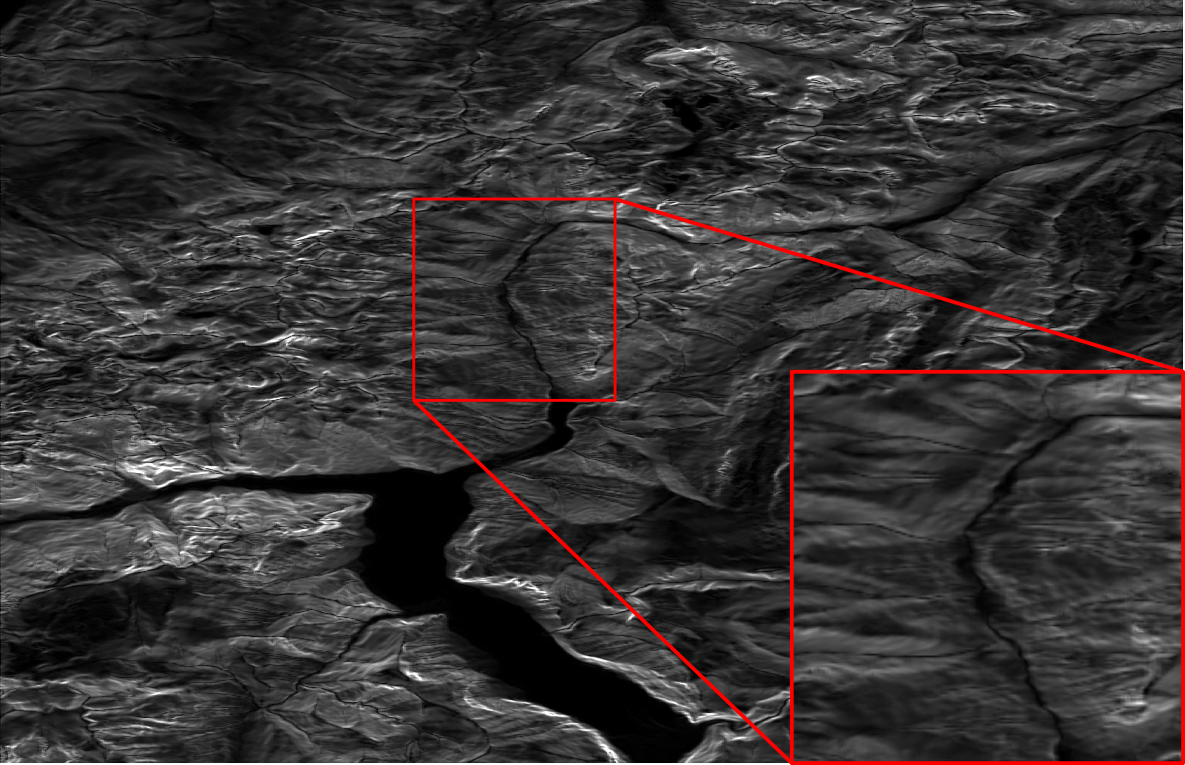
\includegraphics[width=1.0\linewidth]{Resultats/gradient_hauteur.png}
 \caption{Carte de hauteur}
 \end{subfigure}
 \begin{subfigure}[t]{0.32\linewidth}
 \centering
 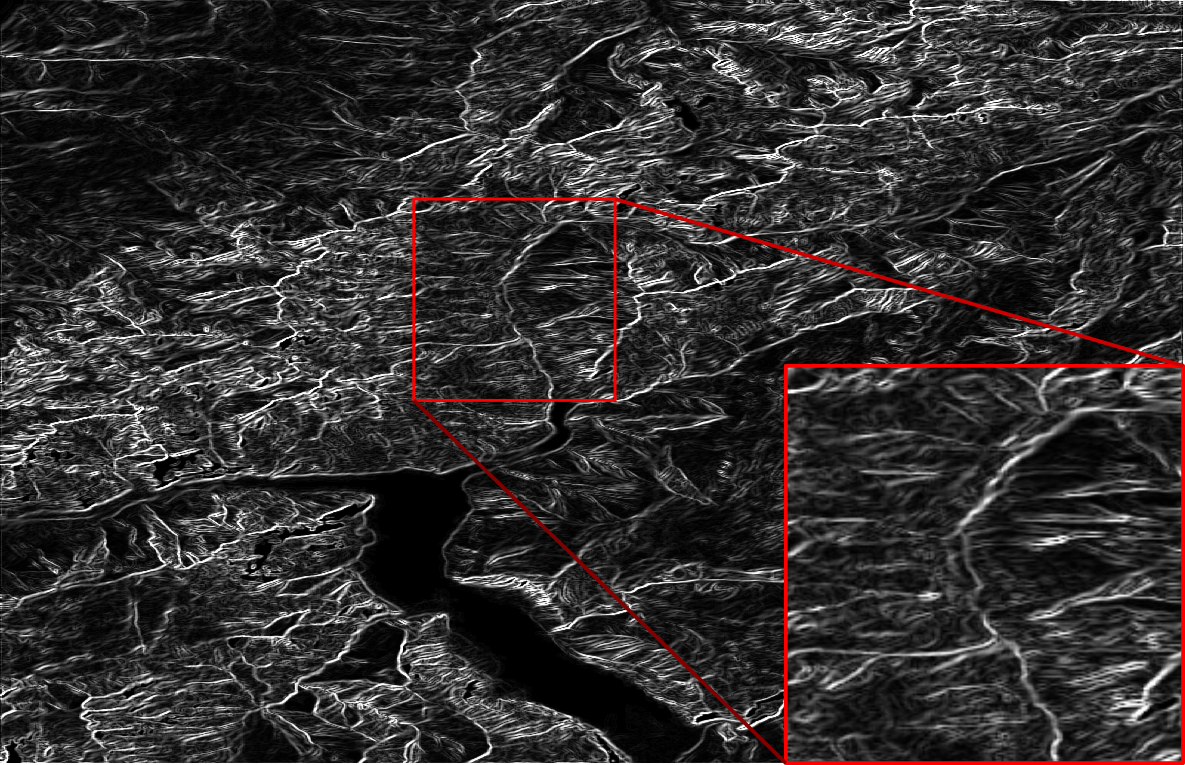
\includegraphics[width=1.0\linewidth]{Resultats/gradient_lambertien.png}
  \caption{Lambertien classique}
 \end{subfigure}
  \begin{subfigure}[t]{0.32\linewidth}
 \centering
 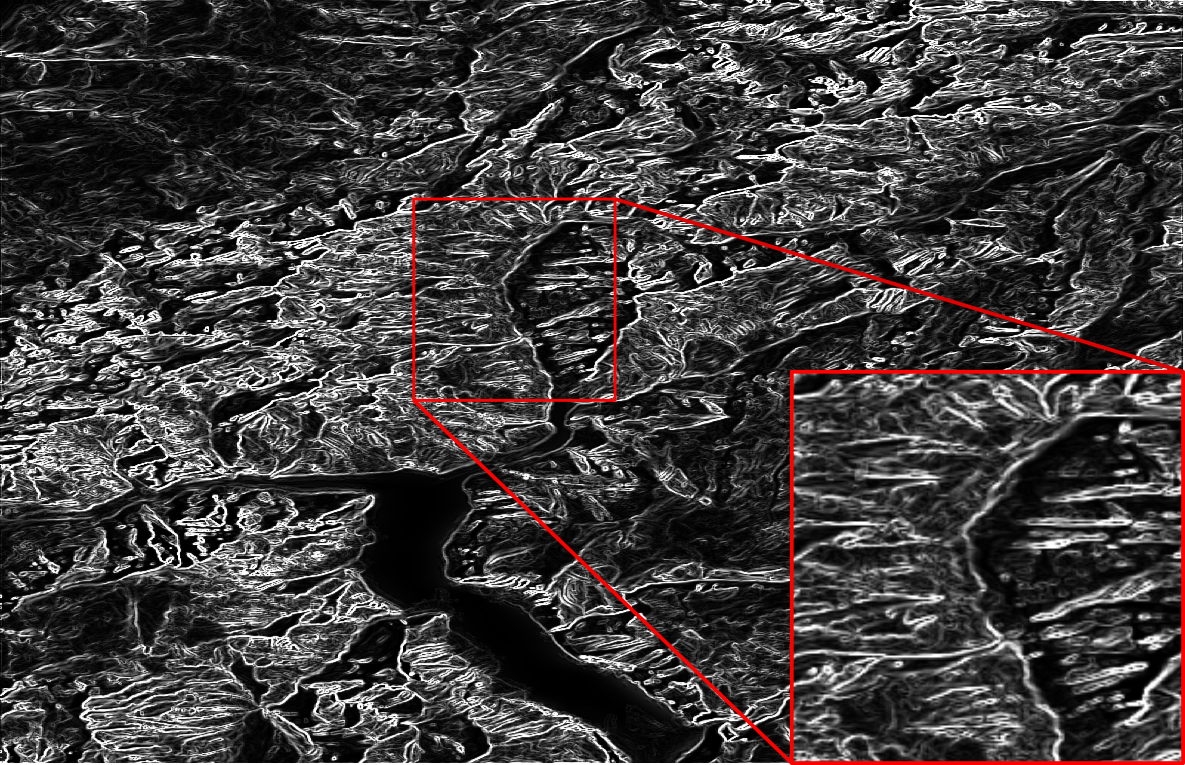
\includegraphics[width=1.0\linewidth]{Resultats/gradient_our.png}
  \caption{Notre méthode d'ombrage}
 \end{subfigure}
 \caption{\label{fig:comparaisonGradient} Comparaison du gradient de la carte de hauteur avec les gradients de l'ombrage d'un Lambertien et de notre méthode ($\alpha = 45\degres$ (Nord-Ouest), $\gamma_o = 45\degres$, $\sigma = 30$). Nous observons que le gradient de notre méthode a des crêtes plus marquées que dans le Lambertien sans pour autant en rajouter par rapport à la carte de hauteur.}
\end{figure*}

\section{Test sur des utilisateurs}

Une dernière validation possible, mais uniquement faisable quand le rendu sera complet, serait de reprendre l’étude faite dans le cadre de MECOMO (\cite{balzarini2016effectiveness}) qui étudiait comment les utilisateurs regardent et comprennent les panoramas de l'atelier Novat et de la reproduire avec des panoramas rendus automatiquement. Nous pourrions alors comparer les résultats de ces deux études et donc vérifier la qualité du rendu. 

